%
% File naacl2019.tex
%
%% Based on the style files for ACL 2018 and NAACL 2018, which were
%% Based on the style files for ACL-2015, with some improvements
%%  taken from the NAACL-2016 style
%% Based on the style files for ACL-2014, which were, in turn,
%% based on ACL-2013, ACL-2012, ACL-2011, ACL-2010, ACL-IJCNLP-2009,
%% EACL-2009, IJCNLP-2008...
%% Based on the style files for EACL 2006 by 
%%e.agirre@ehu.es or Sergi.Balari@uab.es
%% and that of ACL 08 by Joakim Nivre and Noah Smith

\documentclass[11pt,a4paper]{article}
\usepackage[hyperref]{naaclhlt2019}
\usepackage{times}
\usepackage{latexsym}
\usepackage{graphicx}

\usepackage{url}

\aclfinalcopy % Uncomment this line for the final submission
%\def\aclpaperid{***} %  Enter the acl Paper ID here

%\setlength\titlebox{5cm}
% You can expand the titlebox if you need extra space
% to show all the authors. Please do not make the titlebox
% smaller than 5cm (the original size); we will check this
% in the camera-ready version and ask you to change it back.

\newcommand\BibTeX{B{\sc ib}\TeX}

\title{Explore The Power of Transfer Learning: BERT for Text Classification}

\author{Haoran Wang \\
  University of Oregon \\
  {\tt hwang8@cs.uoregon.edu} }

\date{}

\begin{document}
\maketitle
\begin{abstract}
BERT is a language model that was created and published in 2018 by Jacob Delvin and Ming-Wei Chang from Google \cite{BERT}. It has taken the NLP landscape by a storm. BERT has been able to achieve state-of-the-art results in a wide variety of NLP tasks. Many researchers have been working on improving BERT in the past two years. As of now, we have  many variations of the original BERT, such as ALBERT, RoBERTa, DistillBERT, and XLM-RoBERTa, etc. Transfer learning on those models have proven to achieve really good results on many different NLP tasks. In this paper, I have found that transfer learning on BERT and XLM-RoBERTa achieve really good result on text classification in comparison to building a simple model like CNN from scratch. My best performed model is a fine-tuned XLM-RoBERTa cross lingual model, which achieves 0.9459 on the test set. As a comparison, the current number one entry on Kaggle is 0.9555.  In order to do training on a very large model like BERT, we will need the help with Google's hardware TPU (tensor processing units). I have found that TPU is about four times faster than GPU. 
\end{abstract}

\section{Introduction}

For this project, I am competing in Jigsaw Multi-lingual Toxic Comment Classification competition hosted by Jigsaw and Google. Jigsaw, formerly known as Google ideas is a unit within Google that tackles emerging threats from online activities to make internet a better place for all. With the increasing usage of social media, cyber bullying has become a real threat, especially to teenagers. Therefore, Jigsaw and Google have dedicated \$50,000 to host this Kaggle competition to explore how different NLP techniques can be used to classify toxic comments.\\
\\
Text classification is like the “hello world” program in NLP. To make it interesting, I will apply transfer learning on pre-trained BERT as well XLM-RoBERTa and compare the result against using BERT as word embeddings and feed them into a CNN to do text classification.\\
\\
In addition to fine-tuning BERT models, I will be using TPUs (tensor processing units) for training. TPUs are developed by Google and they only support Tensorflow natively. To enable PyTorch on TPU, I will need PyTorch/XLA package.

\section{Background}

This section will review the architecture of BERT and XLM-RoBERTa, as well as the concept of Transfer Learning.

\subsection{BERT} 

BERT, short for Bidirectional Encoder Representation from Transformers has two pre-trained models: BERT base and BERT large. BERT base has 12 layers, and around 110 million parameters. BERT large has 24 layers, and around 340 million parameters \cite{BERT}. It is a very large model indeed. Therefore, I will be using BERT base for this project because of limited resources.\\
\\
To understand BERT, we need to first understand how Transformers work. BERT is basically layers of bidirectional Transformer encoders.\\
\\
Transformers consists a number of encoders and decoders. Each encoder and decoder has two layers: a multi-head attention layer and a fully connected feed forward neural network.\\
\\
Multi-head attention is to compute self-attention multiple times in parallel and independently. The outputs are then concatenated and linearly transformed.\\
\\
Now, let us examine what self-attention is. “Self-attention, sometimes called intra-attention, is an attention mechanism relating different positions of a single sequence in order to compute a representation of the sequence. \cite{attention}” Therefore, it helps the encoder to look at other words in the input sentence when encode each word.\\
\\
To calculate self-attention, the encoder will create a query vector, a key vector, and a value vector for the embeddings of different words in the sequence. Next, we will calculate the dot product of the query vector with the key vector for each word of the input sequence against the other words in the sequence. Then, we will divide the dot product by the square root of the dimension of the key vectors, following by a softmax function. Finally we multiply each value vector by the softmax score and sum up the weighted value vectors.\\
\\
Transformers also add positional encoding when encoding each word. BERT’s structure makes BERT different from context-free word embeddings such as  word2vec and GloVe, which just generate a word embedding (vector) for each word regardless of its context. Instead, BERT can generate different word embeddings based on its context. This makes BERT a very powerful language model.\\

\begin{figure}[!htb]
	\centering
	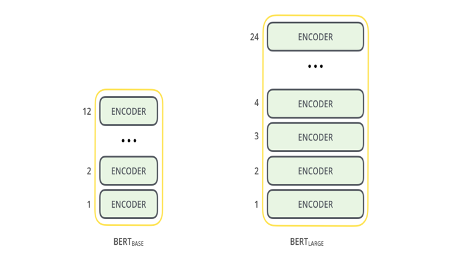
\includegraphics{figures/figure1.png}
	\caption{\label{fig:my-label} BERT base and BERT large \cite{BERT}}
\end{figure}

\begin{figure}[!htb]
	\centering
	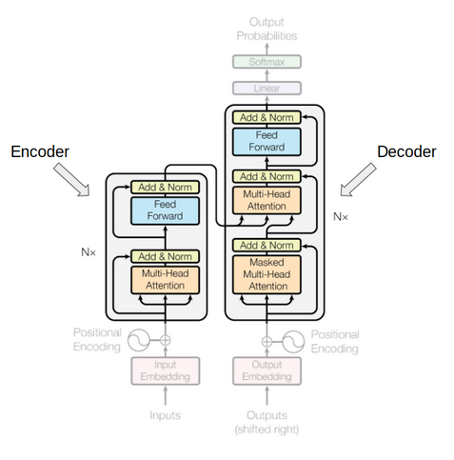
\includegraphics{figures/figure2.png}
	\caption{\label{fig:my-label} Transformer Architecture \cite{attention}}
\end{figure}

\begin{figure}[!htb]
	\centering
	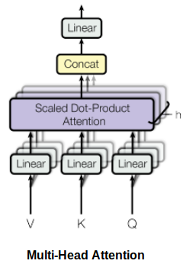
\includegraphics{figures/figure3.png}
	\caption{\label{fig:my-label} Multi-Head Attention \cite{attention}}
\end{figure}


\subsection{Transfer Learning}

Because of how well BERT models performed, transfer learning has come in handy when using BERT to solve different NLP tasks. Instead of building a model from scratch, we can use a pre-trained model like BERT to solve our own spe-cific problem with a little bit fine-tuning to adapt the model to our problem. This saves a lot of resources because our model does not need to learn every parameter from scratch. In the case of pre-trained BERT base, we do not need to learn the first 12 layers of parameters. We can just add a layer on top of them to solve specific problems. \\
\\
So, what tasks are BERT trained on? BERT is pre-trained on two tasks: Masked Language Modeling (MLM) and Next Sentence Prediction (NSP).
For MLM, before feeding text sequences into BERT, some words in the sequence are masked with [MASK] token. BERT then tries to predict the original value of the masked words based on the context of the sequence.
For NSP, BERT receives pairs of text sequences as input, and BERT tries to predict if the second sentence is the subsequent sentence in the original document.
When BERT model was trained, the two tasks were trained together, and the goal was to mini-mize the combined loss function of both tasks.\\


\subsection{XLM-RoBERTa}

BERT is trained entirely on English data. Many researchers who are working on non-English data have then come up with language specific models such as Finish BERT, French BERT and German BERT. However, research on a multilingual model has never stopped. In November, 2019, Facebook AI team resleased XLM-RoBERT \cite{xlm-roberta}, an update to their XLM-100 model. They used RoBERTa \cite{roberta} model (A Robustly Optimized BERT Pretraining Approach) to improve XLM-100 and hence produce XLM-RoBERTa.\\
\\
XLM-RoBERTa is trained on 100 languages, total of 2.5TB of text. The pre-trained XLM-RoBERTa has 550 million parameters, compared to 355 million of RoBERTa.\\

\subsection{TPU}

Tensor Processing Unit is developed by Google to specialize in deep learning. Models that pre-viously take days to train on GPU can be done in hours on TPU. However, in order to use PyTorch on TPU, we have to use a package called XLA, and there are no stable releases yet.\\ 

\section{Data}

This Kaggle competition has provided training set, validation set, and test set. The training set’s comments are entirely in English. The test set’s comments are composed of multiple non-English languages. I have combined the training set from previous competition to make a large training set of 2.1 million comments. Since my resource is limited, I only used the first 200,000 data as my training set. \\
\\
I will use BERT and XLM-RoBERTa pre-trained tokenizer to tokenize and pad the training data. As for the test set, I will use this test set shared by one of the competitors \cite{test-en-df} that translated the entire test set into English. When I evaluate my XLM-RoBERTa model,  I can do it directly without translating the test set because it is a cross-lingual model.\\ 
\\
Since this is a kernel only competition, inferencing is done separately on Kaggle notebook.\\

\section{Models}

This section  investigates three different models.\\

\subsection{BERT for Text Classification Directly}

To adapt pre-trained BERT base model to do text classification, we just need to add a classifier layer on top of the 12 BERT layers. Then, we can fine-tune all the hyper-parameters to improve performance.\\
\\
We will add drop out for BERT base to prevent overfitting. BERT base model produces two outputs: last hidden state and pooler output. After BERT base, we will do a mean pooling and max pooling on the last hidden state from BERT base. Then, we will concatenate them and send it to a linear (output) layer. \\
\\
This linear (output) layer has size of (768*2,1). 768 is the hidden size of BERT base, which means it has 768 output features, we times it by 2 because we did both max pooling and mean pooling before. Since it is a binary classification problem, we put 1 to make the output value between 0 and 1.\\

We will use binary cross entropy with logits loss as our loss function, and Adam with decoupled weight decay\cite{weight} as our optimizer.\\

\begin{figure}[!htb]
	\centering
	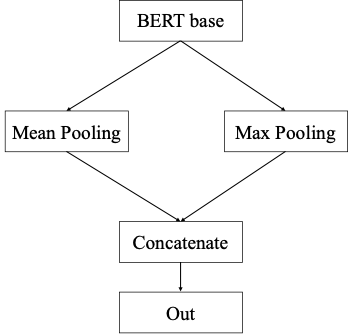
\includegraphics{figures/figure4.png}
	\caption{\label{fig:my-label} BERT for Text Classification}
\end{figure}



\subsection{BERT as word Embeddings + KimCNN}

We will use BERT to tokenize and pad words into word embeddings. Then we will feed those word embeddings to a CNN introduced in this paper \cite{kimcnn} by Yoon Kim from New York Univer-sity in 2014.\\
\\
Here are the steps of how KimCNN works:\\
\\
(1) After we get word embeddings from BERT, which are of size [192, 768]. The max sequence length is 192 and the embedding size is 768.
\\
\\
(2) The model applies convolution on embed-dings that uses three different filters of size [2, 768], [3, 768], and [4, 768]. These filters corre-sponds to capturing the bi-gram, tri-gram, and 4-gram relations.
\\
\\
(3) Apply ReLU to add ability to model nonline-ar problems.\\
\\
(4) Apply 1-max pooling to down-sample the input representation and to help prevent overfit-ting.
\\
\\
(5) Concatenate vectors after 1-max pooling to a single vector.
\\
\\
(6) A dropout layer to help overfitting.
\\
\\
(7) Apply sigmoid function.

\begin{figure}[!htb]
	\centering
	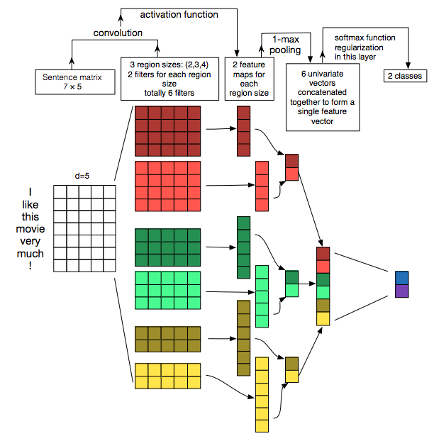
\includegraphics{figures/figure5.png}
	\caption{\label{fig:my-label} KimCNN \cite{kimcnn}}
\end{figure}

\subsection{Cross-lingual model: XLM-RoBERTa}

This is very similar to BERT. The pre-trained XLM-RoBERTa has two outputs, last hidden state and pooler output. The pooler output is feed into a linear layer of size (1024, 1). 1024 is the hidden size of XLM-RoBERTa.

\section{Experiments}

I have fine-tuned BERT and XLM-RoBERTa to compare against CNN. Also, I have trained BERT both on GPU and TPU to compare the performances.\\

\subsection{Fine-tune BERT on GPU}

For fine-tuning, we will tune these hyperparame-ters: learning rate, batch size and number of training epochs.\\
\\
Since our training dataset is rather large and training on GPU takes a long time, we will tune the hyperparameters on the first 50,000 data.\\
\\
The BERT paper had a list of hyperparameters that generally work well across all tasks, which we can use as our starting point to fine-tune \cite{BERT}: 
Batch size: 16, 32; Learning rate: 5e-5, 3e-5, 2e-5; Number of epochs: 2, 3, 4.\\
\\
\textbf {Learning Rate:} Learning rate is perhaps the most critical one of all hyperparameters. To tune learning, rate we fix the training batch size to be 64 and the validation batch size to be 8. Training on one epoch. The training and validation loss plot every 100 batches to make the plot less clustered. We use ROC-AUC score to measure how well our model performs on validation set.\\

\begin{figure}[!htb]
	\centering
	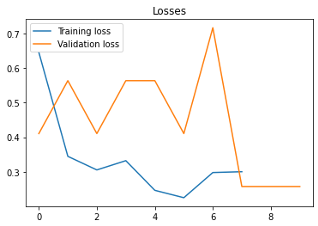
\includegraphics{figures/figure6.png}
	\caption{\label{fig:my-label} Figure 6. lr = 5e-3}
\end{figure}

\begin{figure}[!htb]
	\centering
	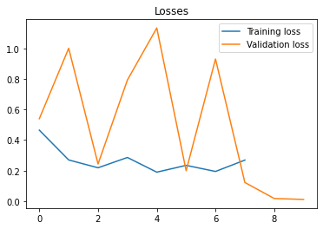
\includegraphics{figures/figure7.png}
	\caption{\label{fig:my-label} Figure 7. lr = 5e-5}
\end{figure}

\begin{figure}[!htb]
	\centering
	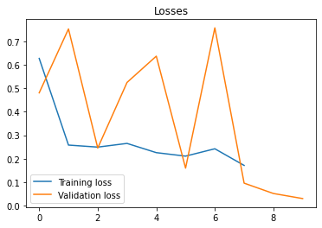
\includegraphics{figures/figure8.png}
	\caption{\label{fig:my-label} Figure 8. lr = 2e-5}
\end{figure}

\begin{figure}[!htb]
	\centering
	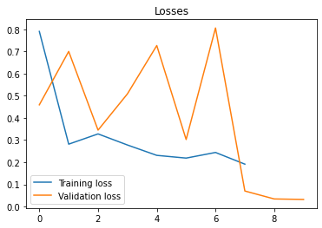
\includegraphics{figures/figure9.png}
	\caption{\label{fig:my-label} Figure 9. lr = 5e-6}
\end{figure}

\begin{table}[!htbp]
	\centering
	\begin{tabular}{|c|c|}
		\hline
		{Learning Rate} & {ROC-AUC} \\ \hline
		5e-3                   & 0.53             \\ \hline
		5e-5                   & 0.82             \\ \hline
		2e-5                   & 0.84             \\ \hline
		5e-6                   & 0.79             \\ \hline
	\end{tabular}
	\caption{Table 1. Learning Rate vs. ROC-AUC}
\end{table}

\noindent As we can see, with an aggressive learning rate of 5e-3, the model did poorly. We find that ideal learning rate should be around 2e-5, which is suggested by the paper.\\
\\

\noindent \textbf {Batch Size:} We will set learning rate to be 1e-5, training on 3 epochs to tune batch sizes.\\
\\
Generally, too large of a batch size will lead to poor generalization, while too small of a batch size will not guarantee to converge to the global optima. It will bounce around the global optima instead. [10]\\
\\
I have found that the max training batch size is 64. I tried training batch size of 128 and 256, which will blow up GPU memory.\\

\begin{table}[!htbp]
	\centering
	\begin{tabular}{|c|c|c|}
		\hline
		{Training} & {Validation} & {ROC-AUC} \\ \hline
		16                           & 2                              & 0.79             \\ \hline
		32                           & 4                              & 0.81             \\ \hline
		64                           & 8                              & 0.82             \\ \hline
	\end{tabular}
	\caption{Table 2. Batch Size vs. ROC-AUC}
\end{table}

\noindent As we can see training batch size of 64 is ideal for this model.\\

\noindent \textbf {Number of Epochs: }  After trained on 6 epochs with learning rate of 1e-6, training batch size of 64, validation batch size of 8. We get an ROC-AUC score of 0.83 at the 6th epoch. As the originial paper suggested, BERT is far less sensitive to hyperparameter tuning on large data sets (100k+)\cite{BERT}. As we can see from the results, once the hyperparameters are set to around the optimal values, it does not affect the model much.\\
\\
\noindent My fine-tuned BERT base model achieved the accuracy of 0.9012 on the test set on Kaggle. This model takes 4.7 hours to train on GPU.\\

\begin{table}[!htbp]
	\centering
	\begin{tabular}{|c|c|}
		\hline
		{Max Sequence Length}   & 192  \\ \hline
		{Training Batch Size}   & 64   \\ \hline
		{Validation Batch Size} & 8    \\ \hline
		{Epochs}                & 5    \\ \hline
		{Learning Rate}         & 1e-6 \\ \hline
	\end{tabular}
	\caption{Table 3. Best Performed BERT}
\end{table}


\subsection{Fine-tune BERT on TPU}

I trained my best BERT model on TPU. I used XLA package, which enables PyTorch on Google TPU. To make the training process even faster, I utilized all 8 cores on TPU to parallel processing. I have trained for one epochs to see how fast the speed up on TPU is.\\

\begin{table}[]
	\centering
	\begin{tabular}{|c|c|}
		\hline
		{XLA : 1} & 12m 16s \\ \hline
		{XLA : 2} & 12m 12s \\ \hline
		{XLA : 3} & 12m 15s \\ \hline
		{XLA : 4} & 12m 13s \\ \hline
		{XLA : 5} & 12m 18s \\ \hline
		{XLA : 6} & 12m 17s \\ \hline
		{XLA : 7} & 12m 28s \\ \hline
		{XLA : 8} & 12m 19s \\ \hline
	\end{tabular}
	\caption{Table 4. Training Time on TPU}
\end{table}

\noindent As we can see, it only takes 12 minutes to train for one epoch on TPU vs. 56 minutes to train for one epoch on GPU.\\

\subsection{BERT + CNN}

Based on my experiments, this model does not perform well on the dataset. The training loss failed to converge to a low rate.

\subsection{Fine-tune XLM-RoBERTa}

After fine-tuning XLM-RoBERTa, my best performed model achieves 0.9459 on test set on Kaggle.\\

\begin{table}[!htbp]
	\centering
	\begin{tabular}{|c|c|}
		\hline
		{Max Sequence Length}   & 192  \\ \hline
		{Training Batch Size}   & 16   \\ \hline
		{Validation Batch Size} & 4    \\ \hline
		{Epochs}                & 2    \\ \hline
		{Learning Rate}         & 5e-6 \\ \hline
	\end{tabular}
	\caption{Table 5. Best Performed XLM-RoBERTa}
\end{table}


\section{Conclusion}

This paper has shown that transfer learning on powerful models like BERT achieves much better result than creating a model from scratch. This is because models like BERT takes a lot of resources to train and it generalize very well on different tasks.\\
\\
Also, I have found that multi-lingual models performs better than mono-lingual models.\\
\\
Lastly, TPU is powerful especially comes to training a very large model like BERT.\\


\newpage
\bibliography{final_report}\
\bibliographystyle{plain}

\end{document}
